% Déclaration du type de document (report, book, paper, etc...)
\documentclass[a4paper, 12pt]{paper} 
 
% Package pour avoir Latex en français
\usepackage[utf8]{inputenc}
\usepackage[T1]{fontenc}
 
% Quelques packages utiles
\usepackage{listings} % Pour afficher des listings de programmes
\usepackage{graphicx} % Pour afficher des figures
\usepackage{amsthm}   % Pour créer des théorèmes et des définitions
\usepackage{amsmath}
\usepackage{microtype} % Optical margins FTW
\usepackage{url}
\usepackage{booktabs} % Allows the use of \toprule, \midrule and \bottomrule in tables for horizontal lines
\usepackage[per-mode=symbol]{siunitx}
\usepackage{floatrow}
\usepackage{caption}
\usepackage{subcaption}
\usepackage{fullpage}
\usepackage{lipsum}



\author{Loïc Amez-Droz \and Florian Reinhard}
\title{Multimode Fibre}

% Début du document
\begin{document}
\begin{titlepage}
\begin{center}
    \textsc{\LARGE École Polytechnique Fédérale de~Lausanne}\\[1.5cm] 
    {\huge \bfseries Optical Engineering: Multimode Fibre}\\[0.4cm] 
    \begin{tabular}{|p{5cm}|p{4cm}|}
        \hline
        Group & C-XX \\ \hline
        Students & Loïc \textsc{Amez-Droz} \newline Florian \textsc{Reinhard} \\ \hline
        Date of lecture & 13.03.2015 \\ \hline
        Date of final report return & 20.03.2015 \\ \hline
    \end{tabular}
\end{center}


\begin{abstract}
    \lipsum[3]
\end{abstract}
 
\vfill
\end{titlepage}

\section{Procedures and results}
\subsection{Evaluation of the numerical aperture with skewed rays}

To determinate the maximum angle of acceptance $\alpha_{max}$, we angle a laser source from the fibre optic axis.
$\alpha_{max}$ is the angle when the circle disappears.

\begin{figure}[H]
    \centering
    \begin{subfigure}[b]{0.45\textwidth}
        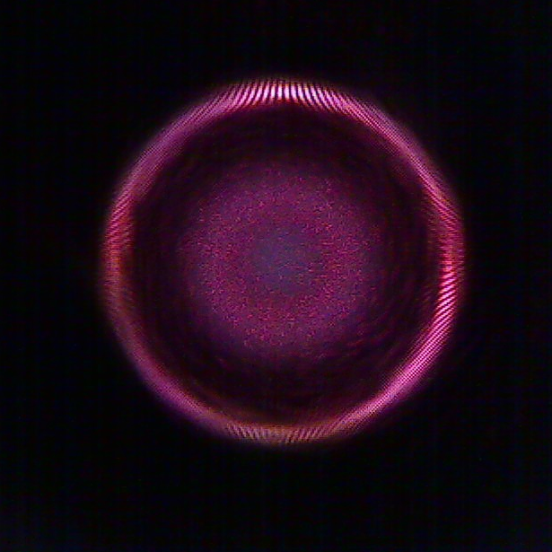
\includegraphics[width=\textwidth]{img/25_deg}
        \caption{Halogen.}
    \end{subfigure}
    \begin{subfigure}[b]{0.45\textwidth}
        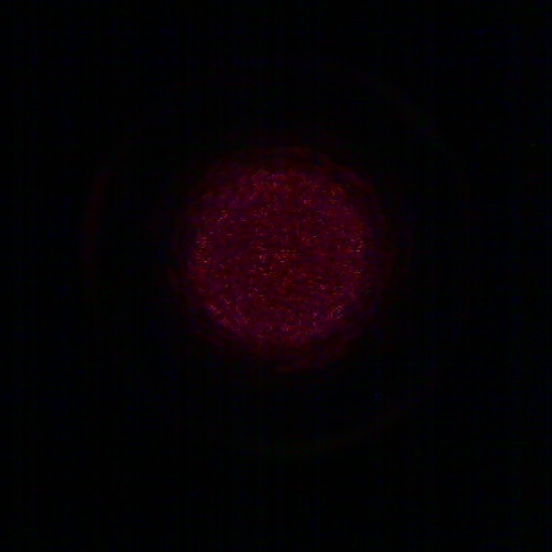
\includegraphics[width=\textwidth]{img/30_deg}
        \caption{LED.}
    \end{subfigure}
    \caption{Injection at different angles to determine the angle of acceptance.}
\label{fig:acceptance_angle}
\end{figure}


The full angle of acceptance $2 \alpha_{max} = \SI{60}{\degree}$.
The center of the beam is still slightly visible after $\SI{30}{\degree}$.
There may be modes that aren't transmitted at the same angle.
The NA is calculated with the acceptance angle $\alpha_{max}$ with an error of $\SI{4}{\degree}$.

\begin{equation}
    \mbox{NA} = n \sin \left( \alpha_{max} \right) = \sin \SI{30}{\degree} = 0.5
    \label{equ:NA}
\end{equation}

\begin{equation}
    \Delta \mbox{NA} = \frac{\partial \mbox{NA}}{\partial \sin \left( \alpha_{max} \right)} \Delta \sin \left( \alpha_{max} \right)= 0.06
    \label{equ:NA_err}
\end{equation}

The datasheet shows $\mbox{NA} = 0.22$.
The circle at $\SI{30}{\degree}$ is just perceptible, therefore the acceptance angle is already passed.
It matches at the angle limit where the intensity of the beam is conserved.
In the picture at $\SI{25}{\degree}$ we can see light between the center beam and the circle.
The angle is small enough so that beams can be transmitted without reflecting.

\subsection{Measurement of the numerical aperture}

We determine the numerical aperture measuring the diameter of the light disk.
The same measurement is made at different distances between the output of the fiber and the sensor.
With the relation between the distance and the diameter we obtained the NA.

\begin{figure}[H]
    \centering
    \begin{subfigure}[b]{0.45\textwidth}
        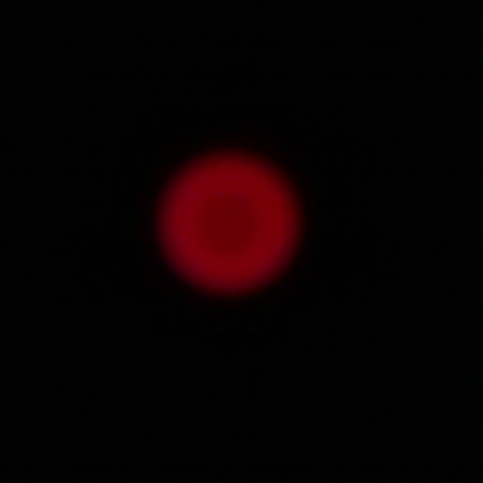
\includegraphics[width=\textwidth]{img/led_0}
        \caption{At fiber exit.}
    \end{subfigure}
    \begin{subfigure}[b]{0.45\textwidth}
        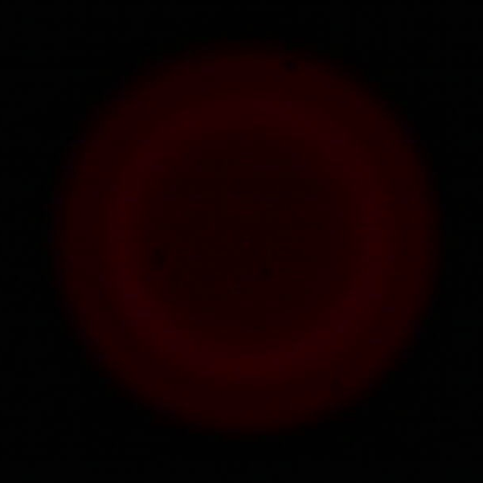
\includegraphics[width=\textwidth]{img/led_2}
        \caption{\SI{2}{\milli\meter} from fiber exit.}
    \end{subfigure}
    \caption{Measurements at different positions relative to the exit of the fiber.}
\label{fig:acceptance_angle_2}
\end{figure}

The diameters $ d_I = \SI{2.835}{\micro\meter} d_{I,px}$ with an error of $\Delta d_{I,px} = 20 \mbox{px}$.

\begin{equation}
    \Delta d_I = \Delta d_{I,px} \frac{\partial d_I}{\partial d_{I,px}} =\SI{56.7}{\micro\meter}
    \label{equ:diam_error}
\end{equation}

\begin{table}[H]
    \centering
    \begin{tabular}{S[table-format=1.1] S[table-format=3.0] S[table-format=1.2]}
        \toprule
        {Relative position (\SI{}{\milli\meter})} & {diameter (px)} & {(\SI{}{\milli\meter})} \\
        \midrule
        0   & 184 & 0.52 \\
        0.5 & 253 & 0.72 \\
        1   & 323 & 0.92 \\
        1.5 & 392 & 1.11 \\
        2   & 449 & 1.27 \\
        2.5 & 524 & 1.49 \\
        3   & 597 & 1.69 \\
        \bottomrule
    \end{tabular}
    \caption{Diameter of the spot at different distances from the fiber exit.}
\label{tab:diams}
\end{table}


\begin{figure}[H]
    \centering
    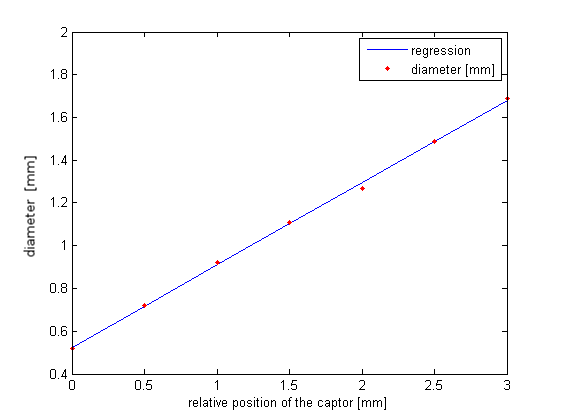
\includegraphics[width=0.8\textwidth]{img/NA_graph}
    \caption{Linear regression of the values in table~\ref{tab:diams} to determine the angle of acceptance.}
    \label{fig:angle_of_a_regression}
\end{figure}

By the linear regression, $\mbox{NA} = 0.36$ with a standard deviation of $\sigma = 0.012$.
It allows to determine the angle of acceptance $\alpha = \SI{21}{\degree}$ and $\Delta \alpha = \SI{1.01}{\degree}$ (which corresponds to $\frac{\alpha}{\Delta \alpha} = \SI{4.8}{\percent}$). 
These values do not correspond to the datasheet.
Maybe we used the wrong fiber in the experiment or we measured wrong.
Another possibility is that we measured light that was injected in the cladding of the fiber instead of the core.

% Source injection
\subsection{Injection for different sources}

\begin{figure}[H]
    \centering
    \begin{subfigure}[t]{0.30\textwidth}
        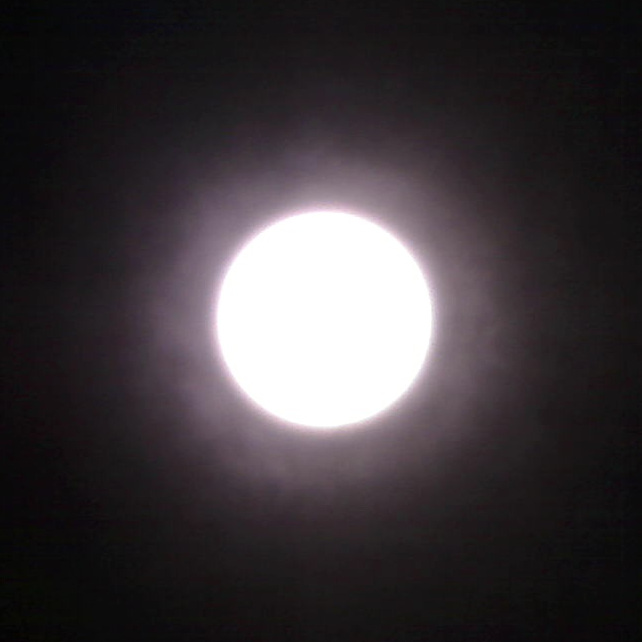
\includegraphics[width=\textwidth]{img/halogen-injection.jpg}
        \caption{Halogen. The halo is due to light being injected into the cladding.}
    \end{subfigure}
    ~
    \begin{subfigure}[t]{0.30\textwidth}
        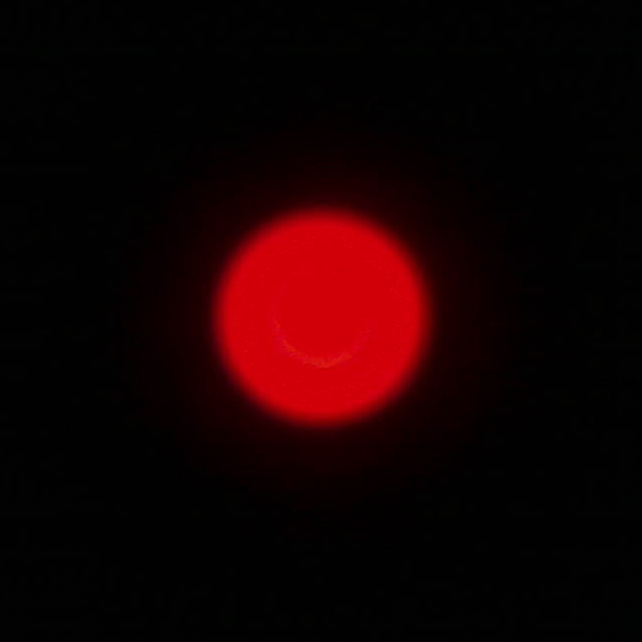
\includegraphics[width=\textwidth]{img/led-injection.jpg}
        \caption{LED. Almost no light in the cladding.}
    \end{subfigure}
    ~
    \begin{subfigure}[t]{0.30\textwidth}
        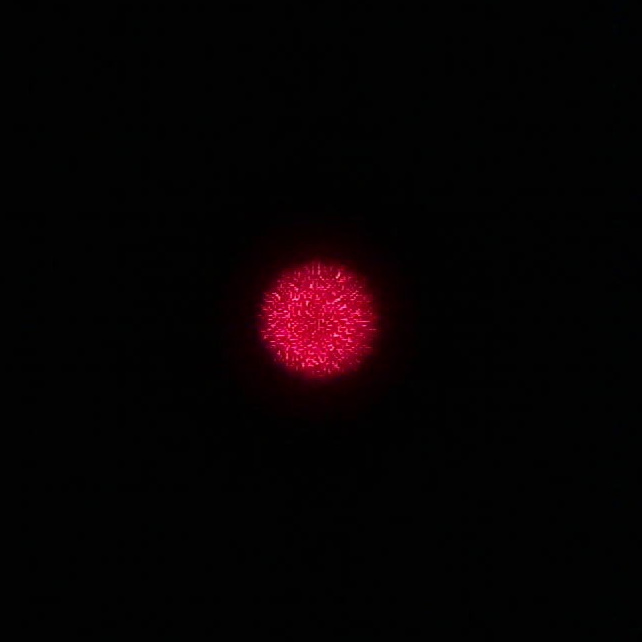
\includegraphics[width=\textwidth]{img/laser-injection.jpg}
        \caption{Laser. The speckles are due to interferences and only appear when injecting coherent light.}
    \end{subfigure}
    \caption{Injection of different sources.}
\label{fig:sources_injection}
\end{figure}


\subsection{Measurement of relative injection efficiency}

We injected the laser source with different \emph{NAs} at the image side and measured the relative intensity over the whole image.
The measurements could have been improved by doing the in a darker room and cooling down the setup to avoid the \emph{dark noise}.

\begin{figure}[H]
    \centering
    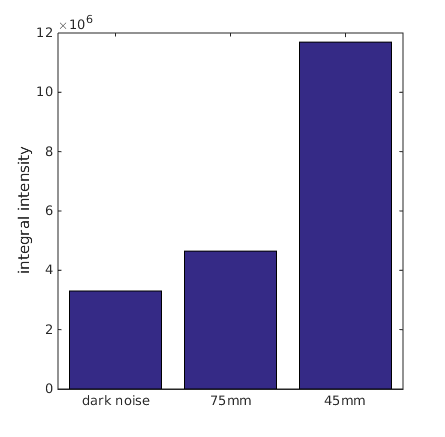
\includegraphics[width=0.5\textwidth]{img/intensity_graph}
    \caption{Integral intensities of two different injection conditions and the dark noise.
        The intensity labeled \emph{45mm} was measured when the light was injected with \emph{higher} NA at the image side.}
    \label{fig:intensity_graph}
\end{figure}

\begin{table}[H]
    \centering
    \begin{tabular}{l S[table-format=1.3]}
        \toprule
        Ratio \emph{without} dark noise correction & 2.516 \\
        Ratio \emph{with} dark noise correction    & 6.244 \\
        \bottomrule
    \end{tabular}
    \caption{Ratios of the integral intensities between the two different injection conditions.
             With and without dark noise correction.}
\label{tab:injection_ratios}
\end{table}

\section{Discussion and conclusions}
Comparing our results to the datasheet for the multimode fiber showed us that our results
were too high. This can be due to a suboptimal setup, injection of light into the cladding, and reflections at the entry of the fiber.
One also might suppose that the datasheet gives a guaranteed angle of acceptance and that some fibers may be slightly better.
\end{document}
